\documentclass[11pt,a4paper]{report}
\usepackage[textwidth=37em,vmargin=30mm]{geometry}
\usepackage{calc,xunicode,amsmath,amssymb,paralist,enumitem,tabu,booktabs,datetime2,xeCJK,xeCJKfntef,listings}
\usepackage{tocloft,fancyhdr,tcolorbox,xcolor,graphicx,eso-pic,xltxtra,xelatexemoji}

\newcommand{\envyear}[0]{2025}
\newcommand{\envdatestr}[0]{2025-04-14}
\newcommand{\envfinaldir}[0]{webdb/2025/20250414/final}

\usepackage[hidelinks]{hyperref}
\hypersetup{
    colorlinks=false,
    pdfpagemode=FullScreen,
    pdftitle={Web Digest - \envdatestr}
}

\setlength{\cftbeforechapskip}{10pt}
\renewcommand{\cftchapfont}{\rmfamily\bfseries\large\raggedright}
\setlength{\cftbeforesecskip}{2pt}
\renewcommand{\cftsecfont}{\sffamily\small\raggedright}

\setdefaultleftmargin{2em}{2em}{1em}{1em}{1em}{1em}

\usepackage{xeCJK,xeCJKfntef}
\xeCJKsetup{PunctStyle=plain,RubberPunctSkip=false,CJKglue=\strut\hskip 0pt plus 0.1em minus 0.05em,CJKecglue=\strut\hskip 0.22em plus 0.2em}
\XeTeXlinebreaklocale "zh"
\XeTeXlinebreakskip = 0pt


\setmainfont{Brygada 1918}
\setromanfont{Brygada 1918}
\setsansfont{IBM Plex Sans}
\setmonofont{JetBrains Mono NL}
\setCJKmainfont{Noto Serif CJK SC}
\setCJKromanfont{Noto Serif CJK SC}
\setCJKsansfont{Noto Sans CJK SC}
\setCJKmonofont{Noto Sans CJK SC}

\setlength{\parindent}{0pt}
\setlength{\parskip}{8pt}
\linespread{1.15}

\lstset{
	basicstyle=\ttfamily\footnotesize,
	numbersep=5pt,
	backgroundcolor=\color{black!5},
	showspaces=false,
	showstringspaces=false,
	showtabs=false,
	tabsize=2,
	captionpos=b,
	breaklines=true,
	breakatwhitespace=true,
	breakautoindent=true,
	linewidth=\textwidth
}






\newcommand{\coverpic}[2]{
    % argv: itemurl, authorname
    Cover photo by #2~~(\href{#1}{#1})
}
\newcommand{\makeheader}[0]{
    \begin{titlepage}
        % \newgeometry{hmargin=15mm,tmargin=21mm,bmargin=12mm}
        \begin{center}
            
            \rmfamily\scshape
            \fontspec{BaskervilleF}
            \fontspec{Old Standard}
            \fontsize{59pt}{70pt}\selectfont
            WEB\hfill DIGEST
            
            \vfill
            % \vskip 30pt
            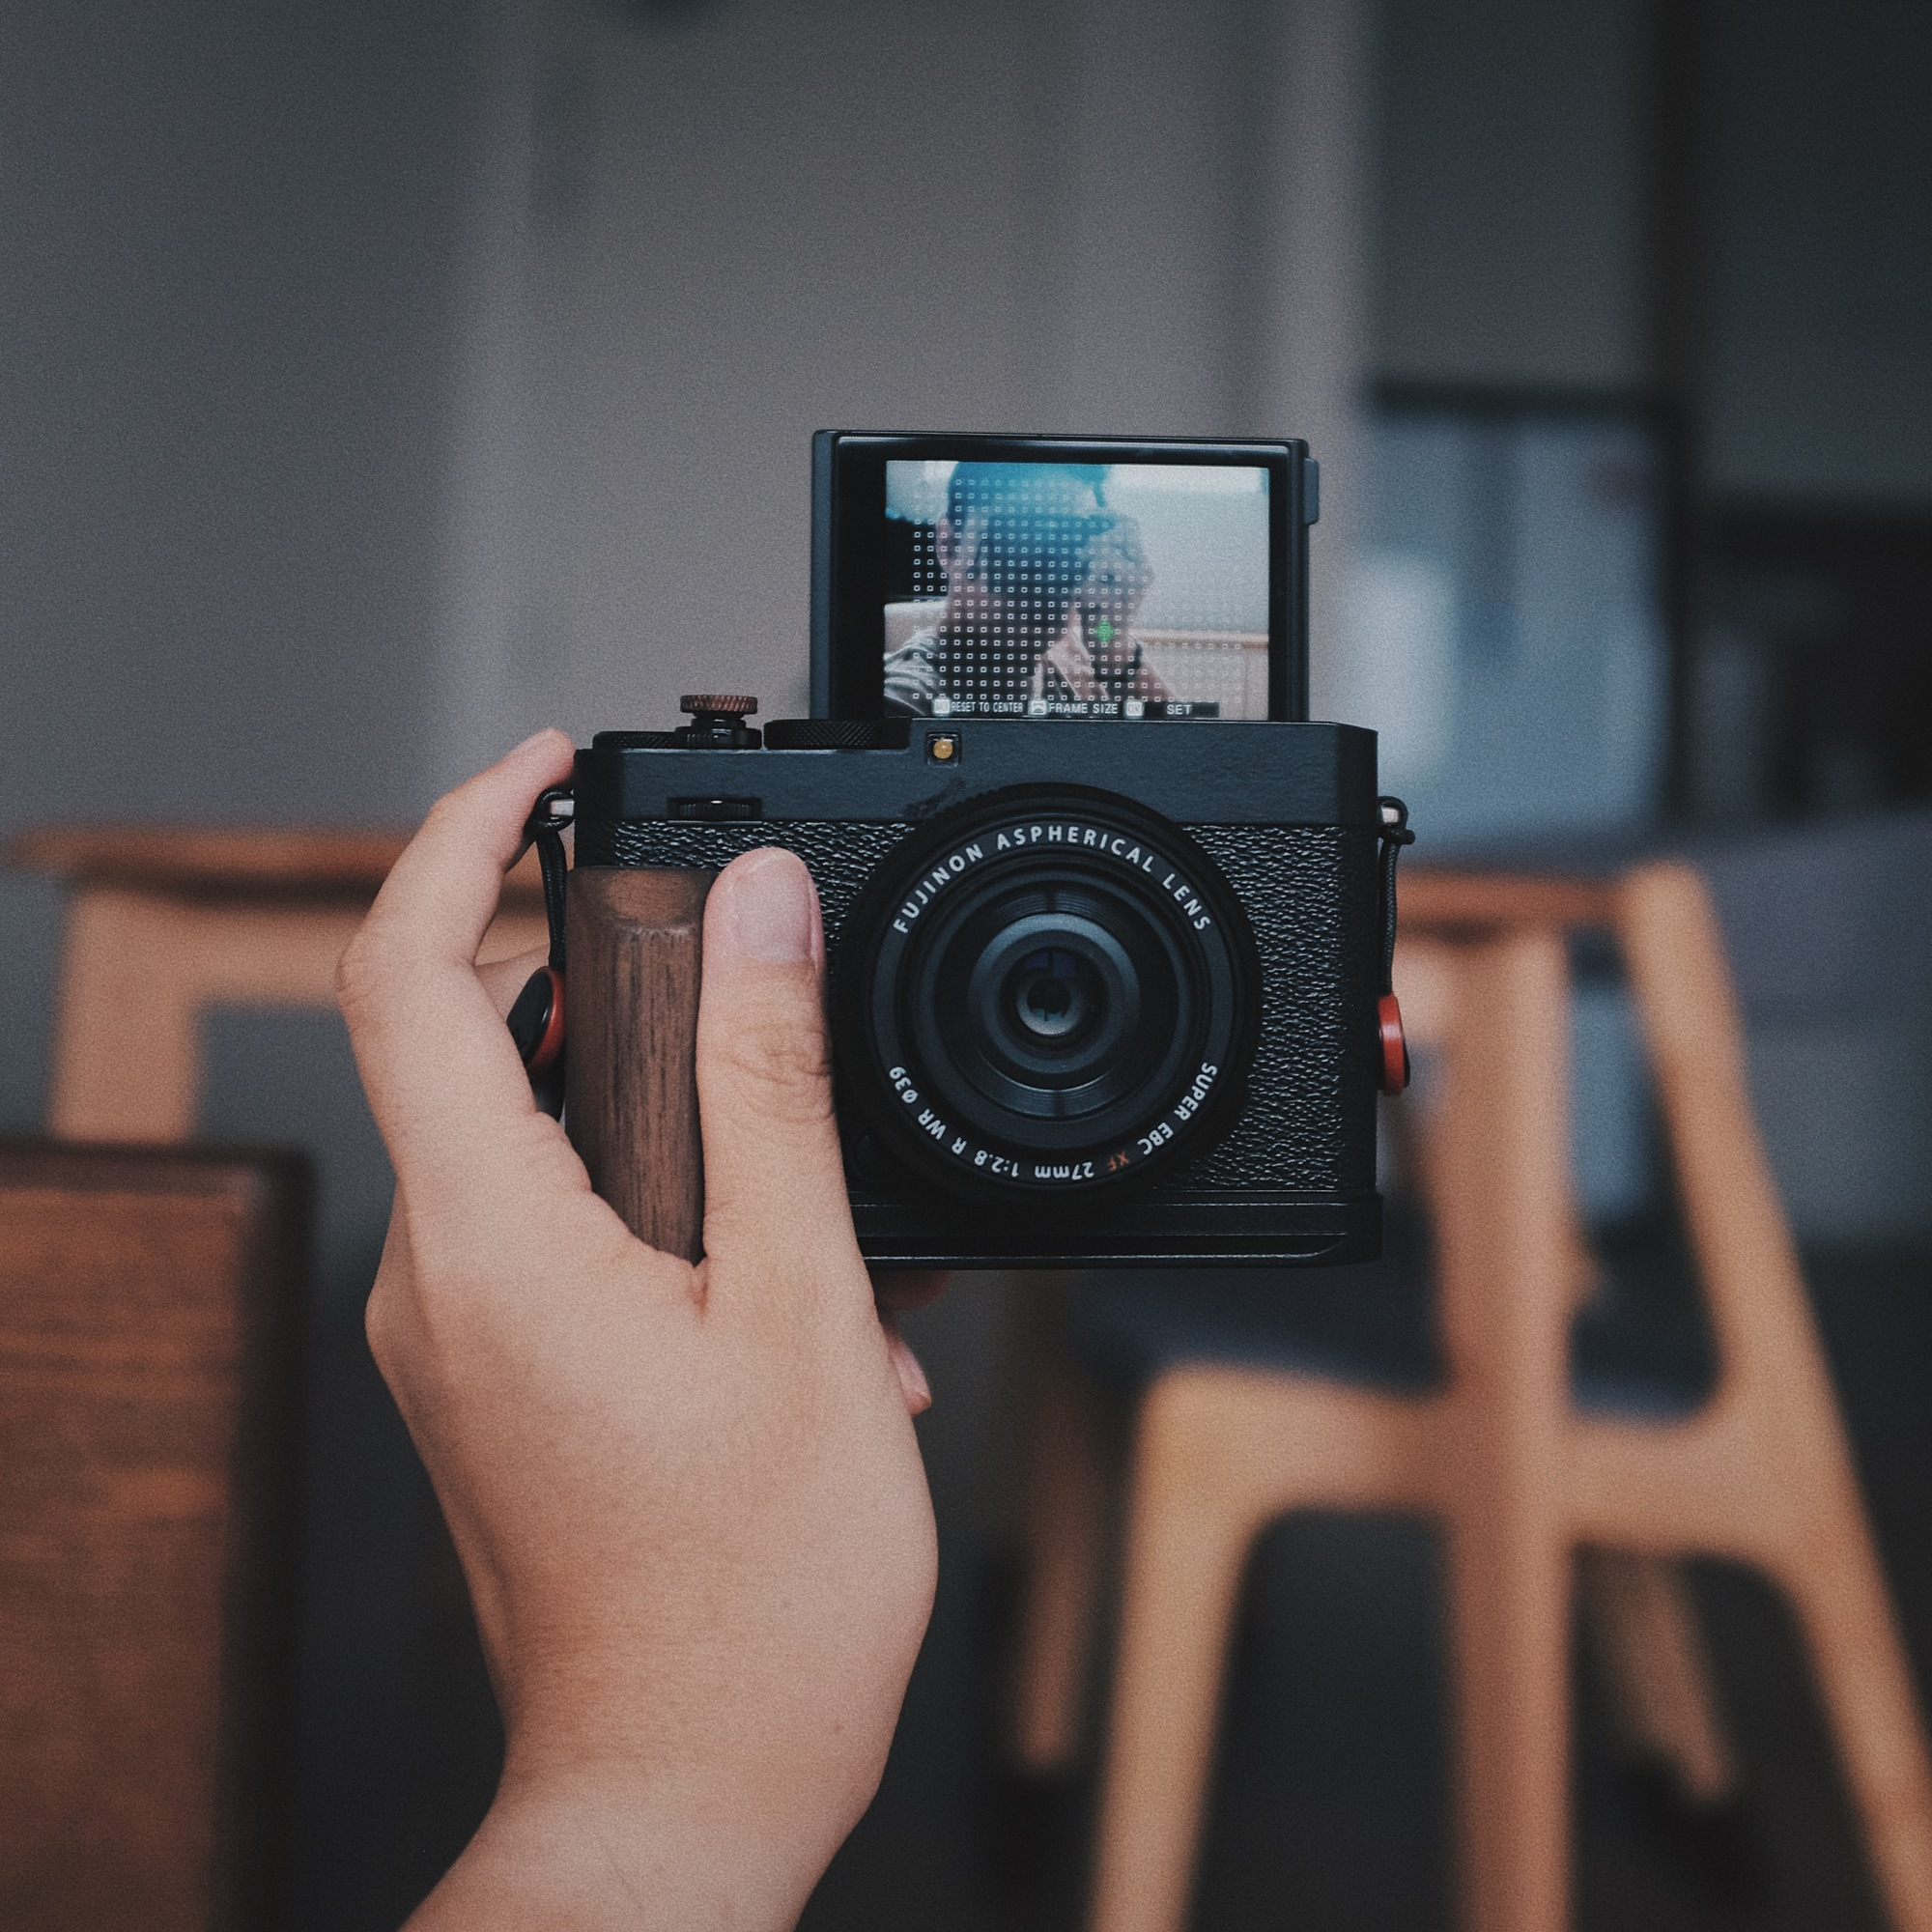
\includegraphics[width=\linewidth]{\envfinaldir/coverpic-prod.jpg}\par
            % \vskip 30pt
            \vfill

            \normalsize\rmfamily\scshape
            \copyright{} The Web Digest Project \hfill\large \envdatestr
        \end{center}
    \end{titlepage}
    % \restoregeometry
}
\newcommand{\simplehref}[1]{%
    \textcolor{blue!80!green}{\href{#1}{#1}}%
}
\renewcommand{\contentsname}{\center\Huge\sffamily\bfseries Contents\par\vskip 20pt}
\newcounter{ipartcounter}
\setcounter{ipartcounter}{0}
\newcommand{\ipart}[1]{
    % \vskip 20pt
    \clearpage
    \stepcounter{ipartcounter}
    \phantomsection
    \addcontentsline{toc}{chapter}{#1}
    % \begin{center}
    %     \Huge
    %     \sffamily\bfseries
    %     #1
    % \end{center}
    % \vskip 20pt plus 7pt
}
\newcounter{ichaptercounter}
\setcounter{ichaptercounter}{0}
\newcommand{\ichapter}[1]{
    % \vskip 20pt
    \clearpage
    \stepcounter{ichaptercounter}
    \phantomsection
    \addcontentsline{toc}{section}{\numberline{\arabic{ichaptercounter}}#1}
    \begin{center}
        \Huge
        \sffamily\bfseries
        #1
    \end{center}
    \vskip 20pt plus 7pt
}
\newcommand{\entrytitlefont}[1]{\subsection*{\raggedright\Large\sffamily\bfseries#1}}
\newcommand{\entryitemGeneric}[2]{
    % argv: title, url
    \parbox{\linewidth}{
        \entrytitlefont{#1}\par\vskip 5pt
        \footnotesize\ttfamily\mdseries
        \simplehref{#2}
    }\vskip 11pt plus 11pt minus 1pt
}
\newcommand{\entryitemGithub}[3]{
    % argv: title, url, desc
    \parbox{\linewidth}{
        \entrytitlefont{#1}\par\vskip 5pt
        \footnotesize\ttfamily\mdseries
        \simplehref{#2}\par\vskip 5pt
        \small\rmfamily\mdseries#3
    }\vskip 11pt plus 11pt minus 1pt
}
\newcommand{\entryitemAp}[3]{
    % argv: title, url, desc
    \parbox{\linewidth}{
        \entrytitlefont{#1}\par\vskip 5pt
        \footnotesize\ttfamily\mdseries
        \simplehref{#2}\par\vskip 5pt
        \small\rmfamily\mdseries#3
    }\vskip 11pt plus 11pt minus 1pt
}
\newcommand{\entryitemHackernews}[3]{
    % argv: title, hnurl, rawurl
    % \parbox{\linewidth}{
    %     \entrytitlefont{#1}\par\vskip 5pt
    %     \footnotesize\ttfamily\mdseries
    %     \simplehref{#3}\par
    %     \textcolor{black!50}{\href{#2}{#2}}
    % }\vskip 11pt plus 11pt minus 1pt
    \begin{minipage}{\linewidth}
            \entrytitlefont{#1}\par\vskip 5pt
            \footnotesize\ttfamily\mdseries
            \simplehref{#3}\par
            \textcolor{black!50}{\href{#2}{#2}}
    \end{minipage}\par\vskip 11pt plus 11pt minus 1pt
}







\begin{document}

\makeheader

\tableofcontents\clearpage




\ipart{Developers}
\ichapter{Hacker News}
\entryitemTwoLinks{Writing my own dithering algorithm in Racket}{https://news.ycombinator.com/item?id=43675309}{https://amanvir.com/blog/writing-my-own-dithering-algorithm-in-racket}

\entryitemTwoLinks{Open guide to equity compensation}{https://news.ycombinator.com/item?id=43675126}{https://github.com/jlevy/og-equity-compensation}

\entryitemTwoLinks{Why Fennel?}{https://news.ycombinator.com/item?id=43673551}{https://fennel-lang.org/rationale}

\entryitemTwoLinks{Skywork-OR1: new SOTA 32B thinking model with open weight}{https://news.ycombinator.com/item?id=43673151}{https://github.com/SkyworkAI/Skywork-OR1}

\entryitemTwoLinks{Half the men in Seattle are never-married singles, census data shows}{https://news.ycombinator.com/item?id=43673125}{https://www.seattletimes.com/seattle-news/data/half-the-men-in-seattle-are-never-married-singles-for-the-first-time/}

\entryitemTwoLinks{Wasting Inferences with Aider}{https://news.ycombinator.com/item?id=43672712}{https://worksonmymachine.substack.com/p/wasting-inferences-with-aider}

\entryitemTwoLinks{The dark side of the Moomins}{https://news.ycombinator.com/item?id=43672593}{https://www.newstatesman.com/culture/books/2025/04/dark-side-of-the-moomins-tove-jansson}

\entryitemTwoLinks{A Reddit bot drove me insane}{https://news.ycombinator.com/item?id=43672139}{https://posthuman.blog/this-reddit-post-fried-my-brain/}

\entryitemTwoLinks{Whenever – typed and DST-safe datetimes for Python}{https://news.ycombinator.com/item?id=43671308}{https://github.com/ariebovenberg/whenever}

\entryitemTwoLinks{Problems with Go channels (2016)}{https://news.ycombinator.com/item?id=43670373}{https://www.jtolio.com/2016/03/go-channels-are-bad-and-you-should-feel-bad/}

\entryitemTwoLinks{How to not build a two stage model rocket}{https://news.ycombinator.com/item?id=43669981}{https://knowone08.gitbook.io/vgecrocketry}

\entryitemTwoLinks{BPS is a GPS alternative that nobody's heard of}{https://news.ycombinator.com/item?id=43669308}{https://www.jeffgeerling.com/blog/2025/bps-gps-alternative-nobodys-heard}

\entryitemTwoLinks{Experimental release of GrapheneOS for Pixel 9a}{https://news.ycombinator.com/item?id=43669185}{https://grapheneos.social/@GrapheneOS/114327666433966529}

\entryitemTwoLinks{Anubis Works}{https://news.ycombinator.com/item?id=43668433}{https://xeiaso.net/notes/2025/anubis-works/}

\entryitemTwoLinks{YAML: The Norway Problem (2022)}{https://news.ycombinator.com/item?id=43668290}{https://www.bram.us/2022/01/11/yaml-the-norway-problem/}

\entryitemTwoLinks{WebTUI – A CSS Library That Brings the Beauty of Terminal UIs to the Browser}{https://news.ycombinator.com/item?id=43668250}{https://webtui.ironclad.sh}

\entryitemTwoLinks{I ditched my laptop for a pocketable mini PC and a pair of AR glasses}{https://news.ycombinator.com/item?id=43668192}{https://www.tomsguide.com/computing/i-ditched-my-laptop-for-a-pocketable-mini-pc-and-a-pair-of-ar-glasses-heres-what-happened}

\entryitemTwoLinks{Zod v4 Beta}{https://news.ycombinator.com/item?id=43667925}{https://v4.zod.dev/v4}

\entryitemTwoLinks{Ask HN: How do you monetize personal code if it's not an "app"?}{https://news.ycombinator.com/item?id=43667887}{https://news.ycombinator.com/item?id=43667887}

\entryitemTwoLinks{Show HN: memEx, a personal knowledge base inspired by zettlekasten and org-mode}{https://news.ycombinator.com/item?id=43667061}{https://gitea.bubbletea.dev/shibao/memex}\ichapter{Phoronix}
\entryitemGeneric{\hskip 0pt{}Linux 6.15-rc2 Released With An Assortment Of Fixes}{https://www.phoronix.com/news/Linux-6.15-rc2-Released}

\entryitemGeneric{\hskip 0pt{}Amarok 3.3 Beta Released For Qt6-Powered KDE Music Player}{https://www.phoronix.com/news/Amarok-3.3-Beta}

\entryitemGeneric{\hskip 0pt{}Intel TDX Support For KVM Finally Expected To Debut In Mainline Linux 6.16}{https://www.phoronix.com/news/Intel-TDX-For-KVM-Linux-6.16}

\entryitemGeneric{\hskip 0pt{}Pinta 3.0 Image Editing Program Released With Port To GTK4}{https://www.phoronix.com/news/Pinta-3.0-Released}

\entryitemGeneric{\hskip 0pt{}DragonFlyBSD Lands "Next-Gen" Disk Encryption Code}{https://www.phoronix.com/news/DragonFlyBSD-DM-Crypt-NG}

\entryitemGeneric{\hskip 0pt{}Qualcomm USB Audio Offloading Poised For Linux 6.16 After Going Through 38 Revisions}{https://www.phoronix.com/news/Linux-6.16-QCOM-USB-Audio-OLOAD}

\entryitemGeneric{\hskip 0pt{}SDL Merges Wayland Multi-Seat Support}{https://www.phoronix.com/news/SDL-Merges-Wayland-Multi-Seat}

\entryitemGeneric{\hskip 0pt{}Linux 6.16 Could See AMD SEV-SNP SVSM vTPM Driver Merged For EPYC CPUs}{https://www.phoronix.com/news/Linux-SNP-SVSM-vTPM-Driver-Tip}

\entryitemGeneric{\hskip 0pt{}A Fresh Take On Virtual Swap Space Being Pursued For The Linux Kernel}{https://www.phoronix.com/news/Linux-Virtual-Swap-Space}\ichapter{Dribbble}
\entryitemGeneric{\hskip 0pt{}Chat App - Two Pages of Sketches}{https://dribbble.com/shots/25890352-Chat-App-Two-Pages-of-Sketches}

\entryitemGeneric{\hskip 0pt{}Nite Riot®\_Film Production // Case Study\_Vol.2.0}{https://dribbble.com/shots/25889874-Nite-Riot-Film-Production-Case-Study-Vol-2-0}

\entryitemGeneric{\hskip 0pt{}Lion}{https://dribbble.com/shots/25884438-Lion}

\entryitemGeneric{\hskip 0pt{}Adobe Acrobat Logo Redesign Concept}{https://dribbble.com/shots/25884888-Adobe-Acrobat-Logo-Redesign-Concept}

\entryitemGeneric{\hskip 0pt{}Hollo Logo Design}{https://dribbble.com/shots/25883411-Hollo-Logo-Design}

\entryitemGeneric{\hskip 0pt{}Fintech Web Design \& Landing Page for Puzzle}{https://dribbble.com/shots/25652139-Fintech-Web-Design-Landing-Page-for-Puzzle}

\entryitemGeneric{\hskip 0pt{}Web Design Crypto Trading}{https://dribbble.com/shots/25879747-Web-Design-Crypto-Trading}

\entryitemGeneric{\hskip 0pt{}Monster Pony Wooden toy}{https://dribbble.com/shots/25880300-Monster-Pony-Wooden-toy}

\entryitemGeneric{\hskip 0pt{}Educate AI Logo Design - Letter E, Monogram, Education}{https://dribbble.com/shots/25879659-Educate-AI-Logo-Design-Letter-E-Monogram-Education}

\entryitemGeneric{\hskip 0pt{}Hawkridge}{https://dribbble.com/shots/25877367-Hawkridge}

\entryitemGeneric{\hskip 0pt{}UI Design for Cargo Delivery Company}{https://dribbble.com/shots/25874804-UI-Design-for-Cargo-Delivery-Company}

\entryitemGeneric{\hskip 0pt{}Nite Riot®\_Film Production // Case Study\_Vol.1.0}{https://dribbble.com/shots/25874978-Nite-Riot-Film-Production-Case-Study-Vol-1-0}

\entryitemGeneric{\hskip 0pt{}UltraSlot}{https://dribbble.com/shots/25875506-UltraSlot}

\entryitemGeneric{\hskip 0pt{}Sidekick Ai 3d mascot}{https://dribbble.com/shots/25874949-Sidekick-Ai-3d-mascot}

\entryitemGeneric{\hskip 0pt{}Equati}{https://dribbble.com/shots/25858079-Equati}

\entryitemGeneric{\hskip 0pt{}🔐 Cybersecurity App Landing}{https://dribbble.com/shots/25873133--Cybersecurity-App-Landing}

\entryitemGeneric{\hskip 0pt{}Howzit}{https://dribbble.com/shots/25871668-Howzit}

\entryitemGeneric{\hskip 0pt{}Brainstorm}{https://dribbble.com/shots/25871145-Brainstorm}

\entryitemGeneric{\hskip 0pt{}Medieval H}{https://dribbble.com/shots/25862061-Medieval-H}

\entryitemGeneric{\hskip 0pt{}Boxplates}{https://dribbble.com/shots/25869902-Boxplates}

\entryitemGeneric{\hskip 0pt{}Nord Print Logo Design - Northern Star, Paper, Print, Printing}{https://dribbble.com/shots/25867726-Nord-Print-Logo-Design-Northern-Star-Paper-Print-Printing}

\entryitemGeneric{\hskip 0pt{}Spark illustrations}{https://dribbble.com/shots/25872229-Spark-illustrations}

\entryitemGeneric{\hskip 0pt{}Peach Media Logo Design}{https://dribbble.com/shots/25869696-Peach-Media-Logo-Design}

\entryitemGeneric{\hskip 0pt{}Quill Pen mark}{https://dribbble.com/shots/25871430-Quill-Pen-mark}


\ipart{Developers~~~~(zh-Hans)}
\ichapter{Solidot}
\entryitemGeneric{\hskip 0pt{}德国 UBI 实验未发现参与者会停止工作}{https://www.solidot.org/story?sid=81037}

\entryitemGeneric{\hskip 0pt{}巴黎限制汽车显著改善了空气质量}{https://www.solidot.org/story?sid=81036}

\entryitemGeneric{\hskip 0pt{}Google 新 AI 模型超越了所有竞争对手}{https://www.solidot.org/story?sid=81035}

\entryitemGeneric{\hskip 0pt{}美国对智能手机等豁免征收关税}{https://www.solidot.org/story?sid=81034}

\entryitemGeneric{\hskip 0pt{}恒星如何吞食行星}{https://www.solidot.org/story?sid=81033}

\entryitemGeneric{\hskip 0pt{}280 万德国人从未上网}{https://www.solidot.org/story?sid=81032}

\entryitemGeneric{\hskip 0pt{}天文学家使用哈勃望远镜获得了天王星最精确自转测量}{https://www.solidot.org/story?sid=81031}

\entryitemGeneric{\hskip 0pt{}Facebook 现在变成了 Craigslist}{https://www.solidot.org/story?sid=81030}

\entryitemGeneric{\hskip 0pt{}生活在 4.36 亿年前的古鱼以袁隆平名字命名}{https://www.solidot.org/story?sid=81029}

\entryitemGeneric{\hskip 0pt{}AI 购物应用 CEO 被控欺诈,AI 的背后其实是人}{https://www.solidot.org/story?sid=81028}

\entryitemGeneric{\hskip 0pt{}微软真的准备推出 Recall}{https://www.solidot.org/story?sid=81027}

\entryitemGeneric{\hskip 0pt{}全球塑料回收率仅为 9\%}{https://www.solidot.org/story?sid=81026}

\entryitemGeneric{\hskip 0pt{}台湾澎湖发现的人骨化石被确认来自丹尼索瓦人}{https://www.solidot.org/story?sid=81025}

\entryitemGeneric{\hskip 0pt{}水道残留的抗焦虑药物改变野生鲑鱼的迁徙行为}{https://www.solidot.org/story?sid=81024}

\entryitemGeneric{\hskip 0pt{}英特尔 CPU 可能受中国对美关税政策影响}{https://www.solidot.org/story?sid=81023}

\entryitemGeneric{\hskip 0pt{}任天堂将越南制造的 Switch 2 游戏机几乎全部出口到美国}{https://www.solidot.org/story?sid=81022}

\entryitemGeneric{\hskip 0pt{}2024 年 58\% 的 PC 游戏收入来自微交易}{https://www.solidot.org/story?sid=81021}

\entryitemGeneric{\hskip 0pt{}科学家测量出中微子至今最精确质量上限 0.45 eV }{https://www.solidot.org/story?sid=81020}

\entryitemGeneric{\hskip 0pt{}美国政治措辞日益倾向于个人信念而不是事实}{https://www.solidot.org/story?sid=81019}\ichapter{V2EX}
\entryitemGeneric{\hskip 0pt{}[问与答] 果然早晚不能刷机。}{https://www.v2ex.com/t/1125196}

\entryitemGeneric{\hskip 0pt{}[程序员] 跑 AI 大模型,到底是用 4090 魔改版好还是 Mac studio 好?}{https://www.v2ex.com/t/1125195}

\entryitemGeneric{\hskip 0pt{}[SONY] 闲鱼的 Sony 低于 200 小时的样机靠谱吗?}{https://www.v2ex.com/t/1125194}

\entryitemGeneric{\hskip 0pt{}[程序员] 把 node.js 程序打包成可执行文件,不过只有 10M}{https://www.v2ex.com/t/1125193}

\entryitemGeneric{\hskip 0pt{}[推广] 🔥Lifetime「内购限免」👍 一款支持 iOS 和 Mac 为飞利浦 Hue、HomeKit 和 LIFX 智能灯提供动态场景和音频功能的应用。}{https://www.v2ex.com/t/1125191}

\entryitemGeneric{\hskip 0pt{}[分享发现] mirroralib,可能是 b 站最快的 CDN?}{https://www.v2ex.com/t/1125190}

\entryitemGeneric{\hskip 0pt{}[问与答] 自建 derp 的话是不是就不用搭建 headscale 了}{https://www.v2ex.com/t/1125188}

\entryitemGeneric{\hskip 0pt{}[职场话题] 工作之余在伦敦参加 KubeCon 2025 小记:给想休息 Gap 一周的朋友作参考的旅游长文}{https://www.v2ex.com/t/1125187}

\entryitemGeneric{\hskip 0pt{}[Windows] Windows 下有什么超轻量的浏览器吗,只要能访问内网就行}{https://www.v2ex.com/t/1125186}

\entryitemGeneric{\hskip 0pt{}[YouTube] 简单 5 个步骤,把旧手机 iPhone 通讯录导出到新手机(2025 年超详细图文+内含 youtube 视频教学)}{https://www.v2ex.com/t/1125185}

\entryitemGeneric{\hskip 0pt{}[Firefox] 告别 FireFox,太让人沮丧了。}{https://www.v2ex.com/t/1125184}

\entryitemGeneric{\hskip 0pt{}[macOS] 求 macOS 好用的录音软件,关键录微信通话和电话, wiretap 下架了。无论软件启动顺序总是能录下才是王。。。}{https://www.v2ex.com/t/1125183}

\entryitemGeneric{\hskip 0pt{}[生活] 家里亲戚被说媒了,求求各位评价一下}{https://www.v2ex.com/t/1125182}

\entryitemGeneric{\hskip 0pt{}[生活] 哪种材质的凉拖鞋能真正做到遇水不臭的?}{https://www.v2ex.com/t/1125181}

\entryitemGeneric{\hskip 0pt{}[生活] 一个人在大城市工作,要做个微创手术,要不要跟父母说?}{https://www.v2ex.com/t/1125180}

\entryitemGeneric{\hskip 0pt{}[求职] 求职 - 远程 remote,后端或全栈开发(有英语口语能力)}{https://www.v2ex.com/t/1125179}

\entryitemGeneric{\hskip 0pt{}[宽带症候群] 上海电信无法获取 ipv6,原生拨号或桥接都不行}{https://www.v2ex.com/t/1125178}

\entryitemGeneric{\hskip 0pt{}[Android] 隐藏小横条模块}{https://www.v2ex.com/t/1125177}

\entryitemGeneric{\hskip 0pt{}[程序员] 618 电脑配置决赛圈}{https://www.v2ex.com/t/1125176}

\entryitemGeneric{\hskip 0pt{}[NAS] PVE8.4.0 直通 Ryzen 4300G APU 核显问题}{https://www.v2ex.com/t/1125175}

\entryitemGeneric{\hskip 0pt{}[React] 有没有熟悉 react native 的老哥,求帮忙看个问题}{https://www.v2ex.com/t/1125174}

\entryitemGeneric{\hskip 0pt{}[iOS] iOS 旧短信自动消失,选已知/未知联系人可恢复显示,怎么解决}{https://www.v2ex.com/t/1125173}

\entryitemGeneric{\hskip 0pt{}[程序员] github 账号被标记了,咋解决呢?}{https://www.v2ex.com/t/1125171}

\entryitemGeneric{\hskip 0pt{}[设计] 请问一下大家学设计有什么推荐的信息流}{https://www.v2ex.com/t/1125170}

\entryitemGeneric{\hskip 0pt{}[Visual Studio Code] vscode 终端错误信息跳转到源码失败(无法正确跳转)的正确解决方式}{https://www.v2ex.com/t/1125169}

\entryitemGeneric{\hskip 0pt{}[Surge] Surge5ForMac 拼车}{https://www.v2ex.com/t/1125168}

\entryitemGeneric{\hskip 0pt{}[问与答] HitPaw Univd 在当前国家或地区不可用;}{https://www.v2ex.com/t/1125167}

\entryitemGeneric{\hskip 0pt{}[随想] 很多领域都有某些中成药一样的东西}{https://www.v2ex.com/t/1125166}

\entryitemGeneric{\hskip 0pt{}[GitHub] GitHub 已屏蔽国区 IP}{https://www.v2ex.com/t/1125165}

\entryitemGeneric{\hskip 0pt{}[Android] 依赖 Shizuku 的应用上架总被谷歌拒绝}{https://www.v2ex.com/t/1125164}

\entryitemGeneric{\hskip 0pt{}[硬件] 请教一下,目前有什么适合编程的 mini-PC/laptop + AR glasses 组合吗?}{https://www.v2ex.com/t/1125163}

\entryitemGeneric{\hskip 0pt{}[Go 编程语言] sponge v1.13.1 发布, Go 开发框架 sponge 深度集成 AI 助手,通过框架约束+AI 生成,提升 AI 在业务场景中的实用性}{https://www.v2ex.com/t/1125162}

\entryitemGeneric{\hskip 0pt{}[问与答] 用什么技术方案能最快最低成本实现一个手机屏幕点击功能?}{https://www.v2ex.com/t/1125161}

\entryitemGeneric{\hskip 0pt{}[问与答] dashengpan.com 挂了吗}{https://www.v2ex.com/t/1125158}

\entryitemGeneric{\hskip 0pt{}[问与答] 有哪些好用的视频配字幕工具啊?}{https://www.v2ex.com/t/1125157}

\entryitemGeneric{\hskip 0pt{}[游戏] [打金] 游戏打金真的能赚钱吗?}{https://www.v2ex.com/t/1125156}

\entryitemGeneric{\hskip 0pt{}[问与答] 想给父母换手机,有什么可选的吗}{https://www.v2ex.com/t/1125155}

\entryitemGeneric{\hskip 0pt{}[程序员] Github 主动屏蔽事件全记录及其绕过}{https://www.v2ex.com/t/1125154}

\entryitemGeneric{\hskip 0pt{}[问与答] 我想问, 125\%的关税,可乐会涨价吗}{https://www.v2ex.com/t/1125153}

\entryitemGeneric{\hskip 0pt{}[Android] 非国行 Android 手机有哪些推荐?}{https://www.v2ex.com/t/1125152}

\entryitemGeneric{\hskip 0pt{}[分享发现] 电子阳痿,是好事儿}{https://www.v2ex.com/t/1125150}

\entryitemGeneric{\hskip 0pt{}[酷工作] [广州][外企] 招聘 Java /全栈/自动化测试/BA}{https://www.v2ex.com/t/1125148}

\entryitemGeneric{\hskip 0pt{}[程序员] 新版 iterm2 这个功能如何关闭?谢谢}{https://www.v2ex.com/t/1125147}

\entryitemGeneric{\hskip 0pt{}[问与答] 广东移动有没有不用换号码的便宜套餐?}{https://www.v2ex.com/t/1125146}

\entryitemGeneric{\hskip 0pt{}[Apple] 15.4 下 m4pro 14 寸 14 核心的 mbp 温度}{https://www.v2ex.com/t/1125143}

\entryitemGeneric{\hskip 0pt{}[问与答] Android 手机变为 Carplay 车机?}{https://www.v2ex.com/t/1125142}

\entryitemGeneric{\hskip 0pt{}[推广] [使用 GitHub 注册] Claw 免费容器-部署青龙-每月 5 美金免费额度}{https://www.v2ex.com/t/1125141}

\entryitemGeneric{\hskip 0pt{}[分享创造] [已开源] BiliNote: AI 视频笔记小工具}{https://www.v2ex.com/t/1125140}

\entryitemGeneric{\hskip 0pt{}[程序员] 相传 github 开始主动屏蔽大陆访问?}{https://www.v2ex.com/t/1125139}

\entryitemGeneric{\hskip 0pt{}[生活] 和对象的相处时光怎么过?求活动建议}{https://www.v2ex.com/t/1125137}


\ipart{Generic News}







\clearpage
\leavevmode\vfill
\footnotesize

Copyright \copyright{} 2023-2025 Neruthes and other contributors.

This document is published with CC BY-NC-ND 4.0 license.

The entries listed in this newsletter may be copyrighted by their respective creators.

This newsletter is generated by the Web Digest project.

The newsletters are also delivered via Telegram channel \CJKunderline{\href{https://t.me/webdigestchannel}{https://t.me/webdigestchannel}}.\\
RSS feed is available at \CJKunderline{\href{https://webdigest.pages.dev/rss.xml}{https://webdigest.pages.dev/rss.xml}}.

This newsletter is available in PDF at
\CJKunderline{\href{https://webdigest.pages.dev/}{https://webdigest.pages.dev/}}.

The source code being used to generate this newsletter is available at\\
\CJKunderline{\href{https://github.com/neruthes/webdigest}{https://github.com/neruthes/webdigest}}.

This newsletter is also available in
\CJKunderline{\href{http://webdigest.pages.dev/readhtml/\envyear/WebDigest-20250414.html}{HTML}} and
\CJKunderline{\href{https://github.com/neruthes/webdigest/blob/master/markdown/\envyear/WebDigest-20250414.md}{Markdown}}.


\coverpic{https://unsplash.com/photos/mountains-reflect-in-a-dark-wet-landscape-24h4vWNHjJE}{Karsten Winegeart}


\end{document}
